\section{Validierung}
In diesem Kapitel geht es darum, Anforderungen und Eigenschaften des Aktor- und Sensorbausteins zu testen.
\subsection{Sensorbaustein}
\subsubsection{ESD Test}
Der Sensorbaustein wird wie eine Unterputzsteckdose verbaut und die Frontplatte dient als User-Interface. 
Genauer bedeutet es, dass der Benutzer, die Touchflächen der Frontplatte berühren muss, um mit dem Sensorbaustein zu interagieren. 
Durch das berühren kann es jedoch zu elektrostatischen Entladungen kommen, die der Sensorbaustein überstehen muss.
Deswegen wurde mithilfe eines ESD-Tests, getestet bis zu welchem Prüfschärfegrad, also bis zur welcher Entladespannung der Sensorbaustein funktioniert.
In der Tabelle \ref{tab: ESD_Testablauf} sind die Prüfschärfegrade und deren Spannungen Abgebildet.
Für den Test wurde die Kontaktentladung genommen, mit welcher eine Entladung über einen Finger nachgestellt wird.\\
Der Testablauf war wie folgt:\\
\\
- Beginn beim tiefsten Schärfegrad\\
- 1 Entladung/s\\
- mind. 10 Entladungen, jeweils auf jeder Touchfläche\\

 \begin{figure}[H]
	\centering
	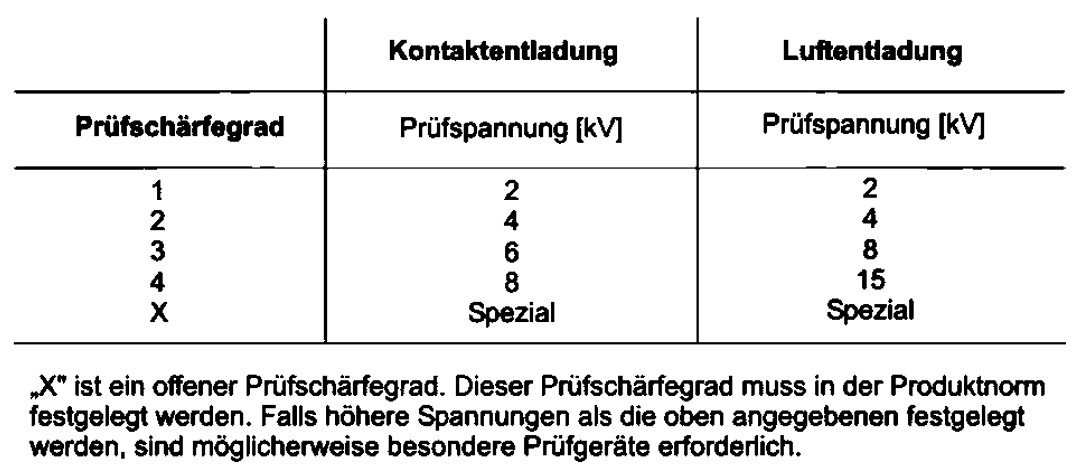
\includegraphics[width=\textwidth]{graphics/ESD_Testablauf.jpg}
	\caption{ESD Testablauf} 	
	\label{tab: ESD_Testablauf}
\end{figure} 


